\chapter*{Original Results}

This chapter contains all the analysis done 
in the original paper and the conclusions that 
it came up with. This is very similar to the original 
paper itself but is redone again to make the compare 
and contrast easier to understand and make the steps 
followed easier to understand.

\section*{System Description}
The following phosphorylation system is used for studying :

\begin{center}
    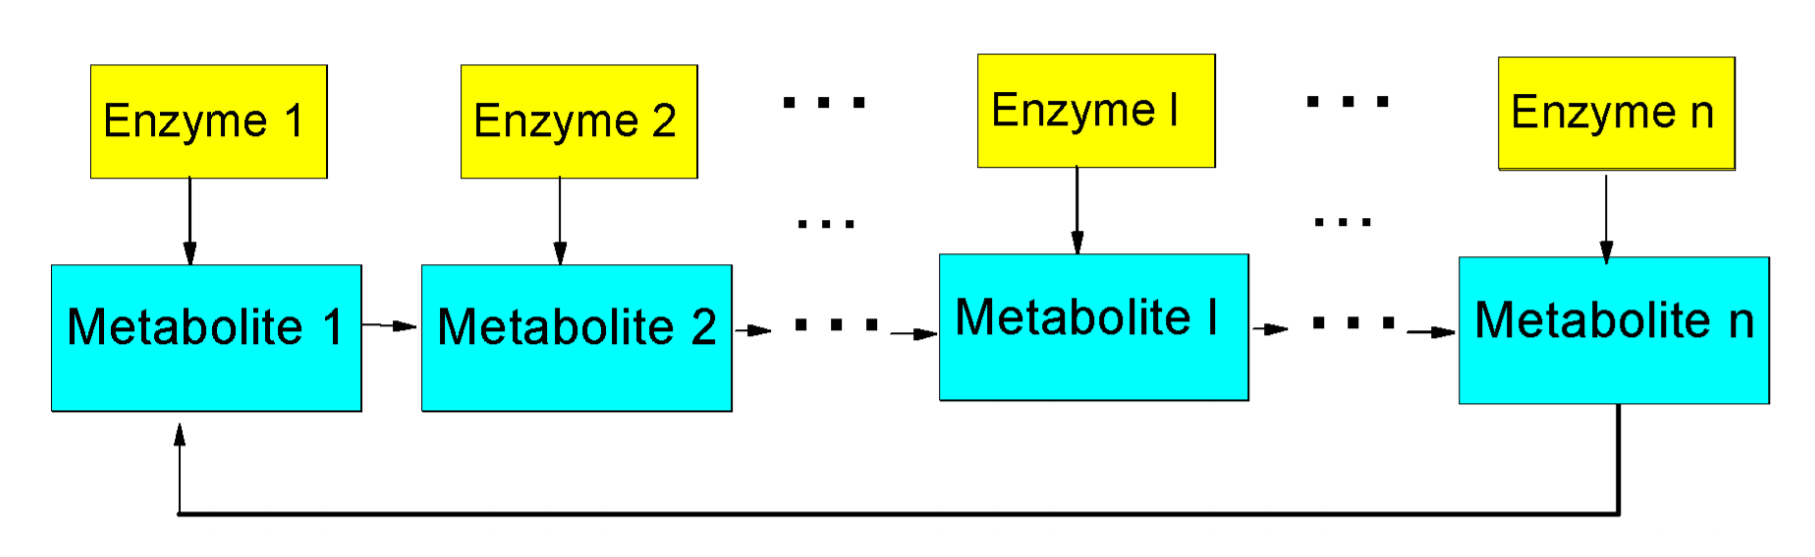
\includegraphics[scale=0.3]{img/orig-sys.png}
\end{center}

\subsection*{Rate Equations}
\noindent This corresponds to the following set of reactions :

$$ \ce{X_i + E_i <=>[K_{i,1}][K_i,2] X_iE_i -> X_{i+1} + E_i}$$

\noindent Which then corresponds to the following rate equations :

\begin{align*}
    \frac{d[X_i]}{dt} &= -K_{i,1}[X_i][E_i] + K_{i,2}[X_iE_i] + K_{i-1,3}[X_{i-1}E_{i-1}]\\
    \frac{d[E_i]}{dt} &= -K_{i,1}[X_i][E_i] + (K_{i,2} + K_{i,3})[X_iE_i]\\
    \frac{d[X_iE_i]}{dt} &= K_{i,1}[X_i][E_i] - (K_{i,2} + K_{i,3})[X_iE_i]
\end{align*}

\noindent As the amount of enzyme remains constant in the 
system, the equations can be rewritten as follows :

\begin{align*}
    \frac{d[X_i]}{dt} &= -K_{i,1}[X_i][X_iE_i] + K_{i,2}[X_iE_i] + K_{i-1,3}[X_{i-1}E_{i-1}] + K_{i,1}[X_i][E_i]_0\\
    \frac{d[E_i]}{dt} &= -K_{i,1}[X_i][X_iE_i] + (K_{i,2} + K_{i,3})[X_iE_i] + K_{i,1}[X_i][E_i]_0 \\
    \frac{d[X_iE_i]}{dt} &= K_{i,1}[X_i][X_iE_i] - (K_{i,2} + K_{i,3})[X_iE_i] - K_{i,1}[X_i][E_i]_0
\end{align*}

\noindent This is due to the fact that $[E_i]_0 = [E]_i + 
[X_iE_i]$, which can be used to eliminate the $[E_i]$ term 
from the equations. 

\subsection*{Allosteric Binding and Negative Autoregulation}
The paper then goes on to describe the phosphorylation 
cycle with allosteric binding and negative autoregulation. 
The reaction taken to exhibit this phenomenon is the
$\ce{DNA -> mRNA -> Proteins}$, where negative 
autoregulation is described.
\\\\
The paper assumes that autoregulation is done by a reversible 
binding/releasing of free and bound promoters, which is 
described below.

$$ \ce{FP + E_{1total} <=>[K_{allo}][K_{rel}] BP} $$

\noindent In this $FP$ is the free promoter and $BP$ is the 
bound one. The assumption that number of binding sites on 
promoters is very small as compared to concentration of 
proteins, to neglect the effect of binding/releasing 
reaction on the dynamics of the enzyme, is also made.
\\\\
The state equations for these reactions are as follows :

\begin{align*}
    \frac{d[FP]}{dt} &= K_{rel}([FP]_{max} - [FP])\\
    \frac{d[mRNA]}{dt} &= K_{pro}[FP] - K_d[mRNA]\\
    \frac{d[E1]_{total}}{dt} &= K_{tran}[mRNA] - K_{allo}\frac{[X_l][E_1]_{total}}{K_{half} + [E_1]_{total}}
\end{align*}
\newpage
\noindent These equations are for the following reaction :

\begin{center}
    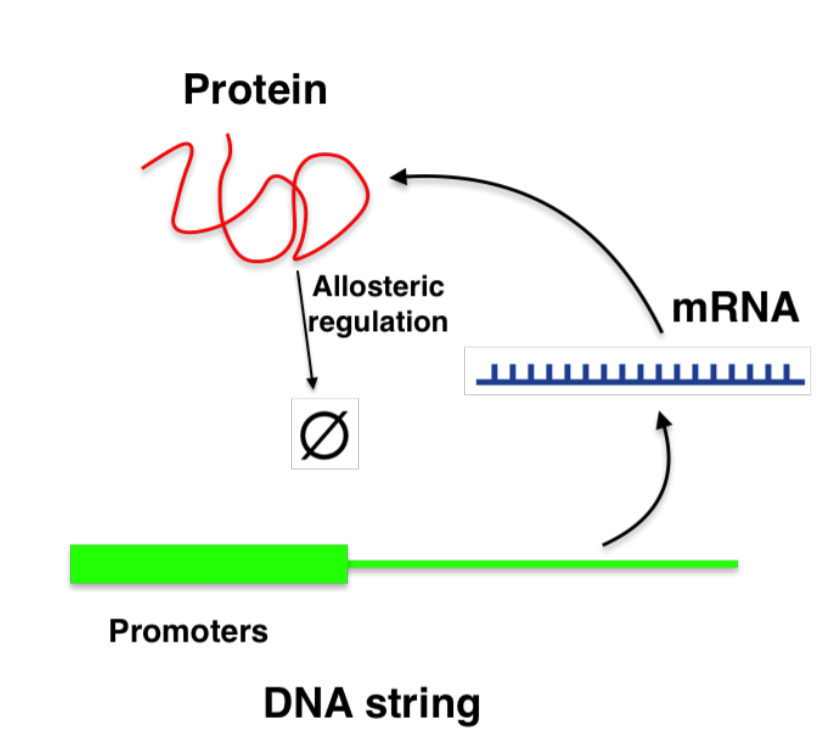
\includegraphics[scale=0.4]{img/dna-noneg.png}
\end{center}

\noindent Another mechanism with negative autoregulation is 
also described by the paper, which is given as follows :

\begin{center}
    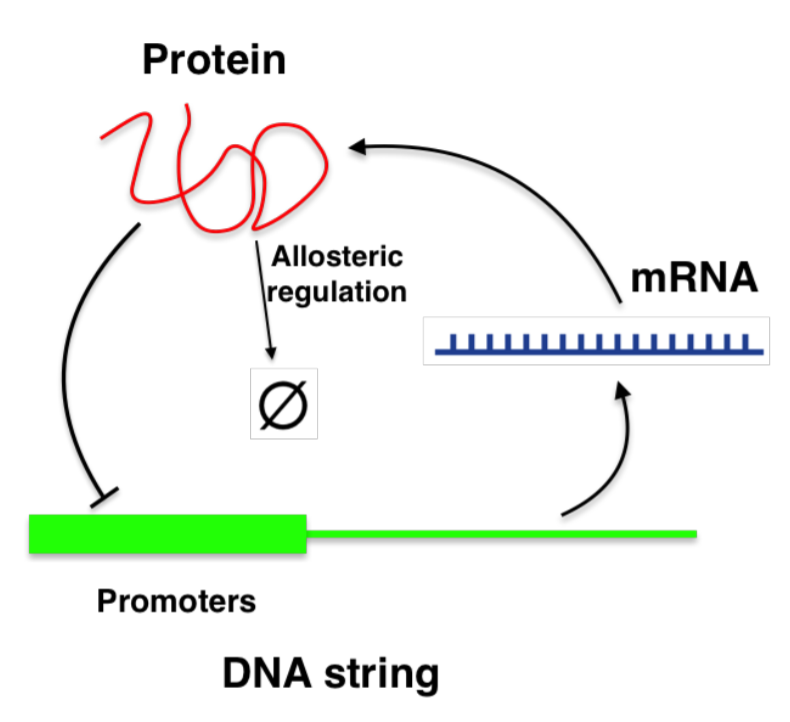
\includegraphics[scale=0.4]{img/dna-neg.png}
\end{center}

\noindent This system is described by the following equations :
\begin{align*}
    \frac{d[FP]}{dt} &= K_{rel}([FP]_{max} - [FP]) - K_{auto}[E_1]_{total}[FP]\\
    \frac{d[mRNA]}{dt} &= K_{pro}[FP] - K_d[mRNA]\\
    \frac{d[E1]_{total}}{dt} &= K_{tran}[mRNA] - K_{allo}\frac{[X_l][E_1]_{total}}{K_{half} + [E_1]_{total}}
\end{align*}

\noindent In these, $[FP]_{max}$ is the total concentration of 
all the promoters.